\documentclass[a4paper,12pt]{article}


\usepackage{amssymb,amsmath,array}
\usepackage{hyperref}
\usepackage{bm}
\usepackage{graphicx}

\usepackage[a4paper, left=3cm, right=2.5cm, top=3cm, bottom=3cm]{geometry}
% language and encoding
\usepackage[utf8]{inputenc}
\usepackage[T1]{fontenc}
\usepackage[english]{babel}
% this package load language specific quotes and enables you to write
% \enquote{text} instead of "`text"' or something like that.
\usepackage{csquotes}
\newcommand{\ts}{\textsuperscript}
\usepackage{caption}

% Write initials inside the right margin
\newcommand{\initials}[1]{\marginpar{\quad\texttt{#1}}}

\title{Report of the 3\ts{rd} project}
\author{Matthias Fedrau (MF), Basel Ammo (BA) \& Linus Behrbohm (LB)}

\date{30\ts{th} January 2021}


\begin{document}

\pagenumbering{gobble}

\pagestyle{myheadings}
\markright{Matthias Fedrau, Basel Ammo, Linus Behrbohm}
    
\maketitle

\begin{center}
    \textbf{Tutorial: Monday 12-14, Tutor: Yasar Plückebaum}
\end{center}
\newpage

\section{Introduction}
\initials{LB}

The data set appears to be a collection of houses represented by 20 attributes e.g. features. The target value is a 1-dimensional floating point value, presumably representing the market price of each house. Because the target values are continuous, we can use regression to predict the price of future houses represented by features of the training data set.

\begin{figure}[!h]
\centering
\begin{minipage}{.3\textwidth}
\resizebox{.6\width}{!}{\begin{tabular}{lrrrr}
\toprule
{} &   Min &     Max &     Mean &     Std \\
\midrule
LotArea       &  1300 &  215245 &  10517.0 &  9978.0 \\
OverallQual   &     1 &      10 &      6.0 &     1.0 \\
OverallCond   &     1 &       9 &      6.0 &     1.0 \\
YearBuilt     &  1872 &    2010 &   1971.0 &    30.0 \\
TotalBsmtSF   &     0 &    6110 &   1057.0 &   439.0 \\
1stFlrSF      &   334 &    4692 &   1163.0 &   386.0 \\
2ndFlrSF      &     0 &    2065 &    347.0 &   436.0 \\
GrLivArea     &   334 &    5642 &   1515.0 &   525.0 \\
FullBath      &     0 &       3 &      2.0 &     1.0 \\
HalfBath      &     0 &       2 &      0.0 &     1.0 \\
BedroomAbvGr  &     0 &       8 &      3.0 &     1.0 \\
TotRmsAbvGrd  &     2 &      14 &      7.0 &     2.0 \\
Fireplaces    &     0 &       3 &      1.0 &     1.0 \\
GarageArea    &     0 &    1418 &    473.0 &   214.0 \\
WoodDeckSF    &     0 &     857 &     94.0 &   125.0 \\
OpenPorchSF   &     0 &     547 &     47.0 &    66.0 \\
EnclosedPorch &     0 &     552 &     22.0 &    61.0 \\
3SsnPorch     &     0 &     508 &      3.0 &    29.0 \\
ScreenPorch   &     0 &     480 &     15.0 &    56.0 \\
PoolArea      &     0 &     738 &      3.0 &    40.0 \\
\bottomrule
\end{tabular}
}
\caption{Inspection of the raw x-value features.}
\end{minipage}
\hfill
\begin{minipage}{.5\textwidth}
\begin{minipage}{1\textwidth}
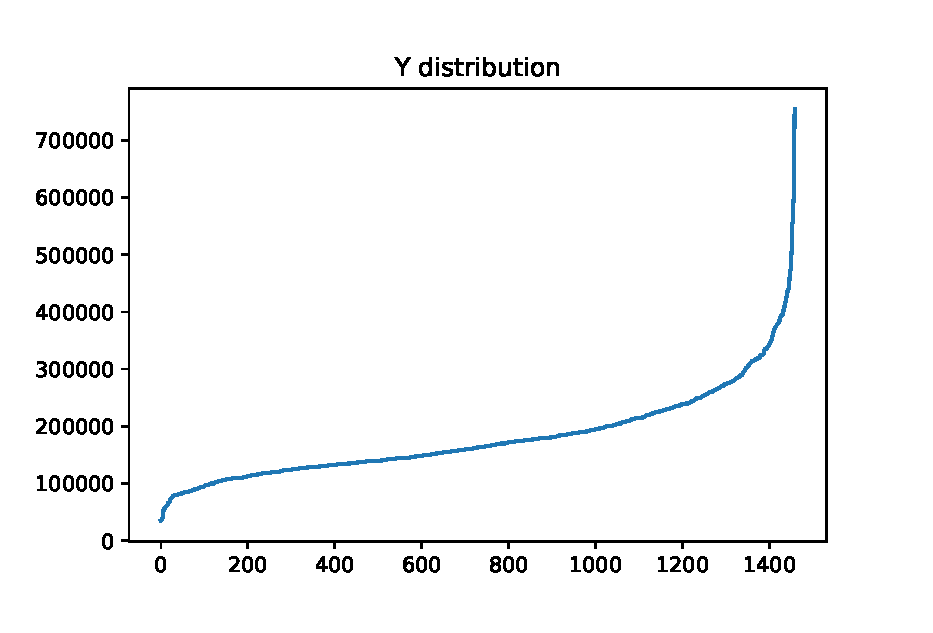
\includegraphics[width=1\textwidth]{plots/y_distribution}
\caption{Sorted y-value distribution. The y-value represents the value of a house.}
\end{minipage}

\vspace{10pt}
\begin{minipage}{1\textwidth}
\resizebox{.6\width}{!}{\begin{tabular}{lllll}
\toprule
{} &      Min &       Max &        Mean &        Std \\
\midrule
y &  [34900] &  [755000] &  [180921.0] &  [79415.0] \\
\bottomrule
\end{tabular}
}
\caption{Inspection of the raw x-value features.}
\end{minipage}
\end{minipage}
\label{fig_res}
\end{figure}

We can see that there are a lot of medium priced houses and a very few very highly priced houses. These few data points will be very important for the training process, as they are very different from most of the other samples. These points could be mistaken as outliers, but should not be ignored as they are presumably legitimate samples of house prices.\\

We can see that the feature set is primarily positively correlated, with some slight negative correlations. We can also see a clear correlation between the target value y and some of the features, which makes them good candidates during feature selection.

\begin{figure}[!h]
\centering
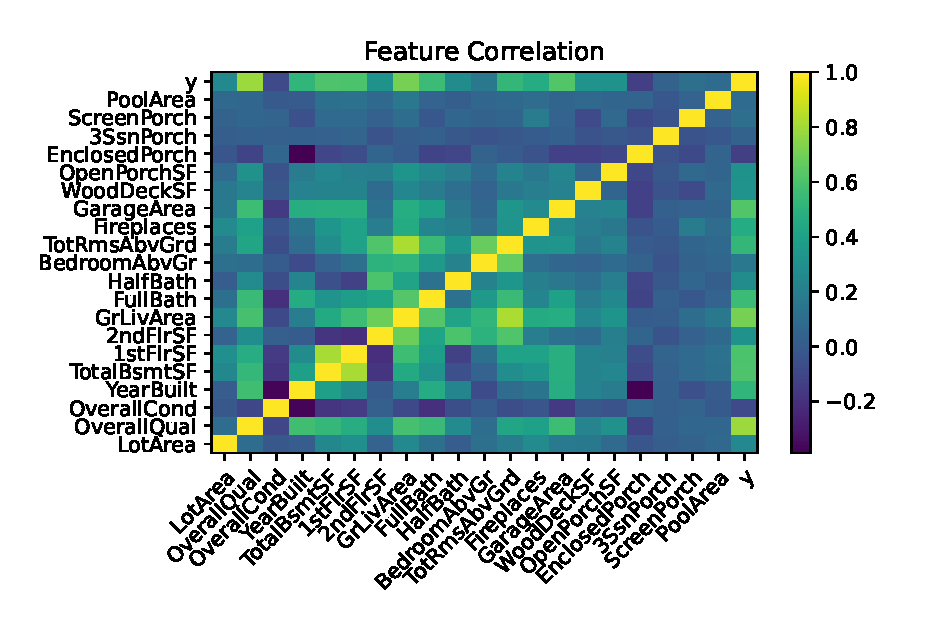
\includegraphics[width=0.6\textwidth]{plots/full_feature_correlation}
\caption{Pairwise correlation of all features and target value.}
\end{figure}

\section{Foundations}
\initials{MF}
\subsection{Methods}
As the name Linear Regression implies, the general assumption is that the relationship between input and output is linear.
Linear regression corresponds to modelling a linear function in feature space, hence for a one dimensional feature vector you get a line, for two-dimensional a plane and so on. To maximize the performance of the model one need a metric to decide between different functions, in case
of Linear Regression its usually done by the distance between the points and the function.
\begin{description}
\item \textbf{Ridge Regression}\\
The indention is to prevent overfitting in linear regression, hence ridge regression is similar to linear regression, but in contrast constraints the weights of the model, more precise the small weights. That leads to flatter curves as the parameter goes up, which prevent overfitting. It uses the regularization L2, which penalizes large model coefficients.
\item \textbf{Huber Regression}\\
The idea here is again to compensate a disadvantage of general linear regression, which is sensitive to outliers. Huber Regression does this by using a regularization made by L1 and L2. Since L1 is more robust to outliers. The general assumption is that all data, that are not in a linear relation are outliers.
\item \textbf{Random forest regressor}\\
A random forest is a meta estimator that fits multiple decision trees to different subsets of the dataset and recombines them. Each decision tree learns a tree of splits in the dataset's feature space, that divides the data in the "purest" way possible. For regressors, this usually means to minimize the weighted average variance across all sections of the split. The split usually only occurs in the space of a single feature. That way, features which explain a lot of the variance can be easily found, which we will later use for feature selection.
\end{description}

\subsection{Preprocessing}
\initials{LB}
We tested different randomization and standardizations of the data. Standardizations we used were standard scaling, robust scaling and L2 normalization.
\begin{description}
\item \textbf{Standard scaling}\\
Transposes all datapoints by subtracting the mean and divides by the standard deviation, resulting in a mean of 0 and a standard deviation of 1.
\item \textbf{Robust scaling}\\
Transposes all datapoints by subtracting the median and divides by the interquantile range (range between 25th and 75th quantile). This avoids effects from extreme datapoints and makes the pipeline less sensitive to outliers.
\item \textbf{L2 Normalization}\\
Divides each datapoint by its L2-norm, scaling their lengths to 1. This removes the information of absolute quantity in feature values and renders datapoints as qualitative vectors, representing only the relations between the features.
\end{description}
We also shuffled the data and evaluated different shufflings to help avoid any drop outs during cross validation.

\subsection{Evaluation}
\initials{LB}
For evaluation of the pipeline we used cross validation using R2 score and negative mean squared error (NMSE). We tried different numbers of cross validation folds between 5 and 100, but settled at 10 folds as it provided a good balance between testing coverage and computation cost.
\\\\
The evaluation of the models is done by R2 and NMSE.
R2 is basically the sum squared error(SSE) divided by the variance of y-true. To obtain a result, which is better the higher the score is, we subtract the prior formula from one.
\\
$$
R^2 = 1 - \frac {\sum_i (f(\vec{x}_i) - y_i)^2} {\sum_i (y_i - \overline{y})^2}
$$
NMSE or negative mean squared error is the negative sum of the squared difference between predictions for y and the true y divided by the number of data points.
$$
\mathit{NMSE} = - \frac{1}{n}\sum_i (f(\vec{x}_i) - y_i)^2
$$

 Later we also used a learning curve to evaluate the learning ability of specific models. In order to do that, we train the model with growing amount of data, starting with one and going up to to total amount of data.
 
\subsection{Feature Selection}
\initials{MF}

\begin{description}
\item \textbf{Filter methods}\\
\textbf{Correlation-based feature selection:} Assigning a weight to every feature on the basis of the correlation between the feature(Xj) and the output(y). The best performing features are then taken for training. Here the range is from all-in-one to complex methods. The methods advantage is the simplicity of the computation, the disadvantage the neglection of the model and the correlation between features.\\
\textbf{Variance Threshold:} This filters features with a very low variance by removing any features with a variance below a threshold. This improves computation performance and makes the model more robust on new data, which might have different values for those features the model can not be trained on.\\
\item \textbf{Wrapper methods}\\
\textbf{Forward selection:} The simple idea here is to remove features and then evaluating the performance of the model. By comparison of the performance with and without the feature/features one can estimate the importance of features and by that the need for them.\\
However Finding the optimal set features is an NP-hard-problem and neglects the correlation between the features, which is a huge drawback, on the other hand this method takes the model into account.\\
\item \textbf{Embedded methods}\\
\textbf{Random Forest:} Learns feature importance while fitting. Those features which reduce the variance in large subsections of the data are assumed to be more important than other features. A decision tree can therefore easily estimate feature importance, by ranking the features with splits near the root of the tree as more important.
\end{description}

\section{Experiments}

\subsection{Set-Up}
\initials{LB}
We started with the assumption that high house prices might be outliers, therefore we take at least one model which is robust to outliers(e.g. Huber) and one which is sensitive to outliers(e.g. Linear Regression).\\
Regarding preprocessing we just take all methods we know from the lecture, and tried them out experimentally.\\
For feature selection, first we used a filter method to quickly remove some of the less important features. We used a variance threshold to remove quasi constant features. Later we used a model with an embedded feature selection, namely a random forest, to determine the most important features of the data set.

\subsection{Results}
\initials{LB & MF}
In our first evaluation round the linear regression and ridge regressor performed equally in all tests. Huber regression, even though very similar to ridge and linear regression, performed the worst and random forest performed the best on average on all data scalings (see Fig. 11 in Appendix).
Of the scalings (see Fig. 7-9) the standard scaling yielded the best results while L2 normalization decreased average model performance compared to the raw data (see Fig. 10).\\
One observation was that during cross validation, there would be major performance drops for single folds. Although L2 normalization decreases the overall performance of the models, it seemed to mitigate the performance drop in these folds (see Fig. 9).\\
To ensure that this performance drop was not a coincidence, we shuffled the data set and confirmed that the performance drop still occurs, only at a different fold during cross validation (see Fig. 6).\\
There is not a lot of difference between the NMSE and R2 scores, but the R2 score performs a little better on the raw data and is more stable during cross validation.\\
During feature selection the filter method (variance threshold) filtered only one feature, \textit{HalfBath}, as it showed a lower variance than 0.3. The random forest selected only very few features as important, as shown in Table 1 in the appendix.\\
The learning curve of random forest(see Fig. 11) flattens quickly, but the slope keeps to be positive. Hence the relation between growing data and improvement in score is not linear.\\
The learning curve of linear regression(see Fig. 12) flattens quickly, moreover it seems to converge to a certain value. Hence the slope is approximately 0 and therefore the model will not improve with growing data after a certain threshold.

\subsection{Analysis}
\initials{LB & MF}
Ridge regression is basically linear regression additionally minimizing its coefficients to prevent overfitting. When the coefficients do not have to become too large to fit to the training data, it behaves just like regular linear regression.\\
The bad performance of Huber Regression might be because of the outlier assumption of the model. Therefore a non-linear relation between the data is possible and large values are not necessarily outliers. The other linear models might perform better, because they also respect the larger data points.\\
The linear models are all performing worse than the random forest, which indicates that there are non-linear relationships between the features and the target value which the linear models can not fit to.\\
The improved stability of the R2 score on the raw data might be due to the R2 scores inclusion of the target value's variance. This causes it to reduce the error component on data sets with highly varying target values.\\
The sudden performance drops during cross validation are probably due to the very few highly priced houses which are very different to most other points in the data set. If they are excluded from the training data set during cross validation, the models will not learn about these data points and their test score drops significantly.\\
L2 normalization seems to be less sensitive to these missing data points, as it shows a smaller much performance drop on the fold where other scalings have large drops. This could be explained by L2 ignoring the length of the data vectors and only learning from their direction, which can be interpreted as the ratios between the data features. Therefore data points with high values overall are not considered as much as the combination of the features and their relationships.

\section{Discussion}
\initials{LB & MF}
Because of the very high variance in the target values of the data set, it is important during cross validation to divide the data set into subsets of data with approximately equal variance as the complete data set. This could be achieved by applying a cross validation strategy which fills each of its folds by taking samples from the complete dataset in an ordered fashion from smallest to largest target value, resulting in cross validation folds with samples from the whole spectrum of the target value distribution.

\newpage
\appendix
\section{Appendix}

\begin{figure}[h]
\centering
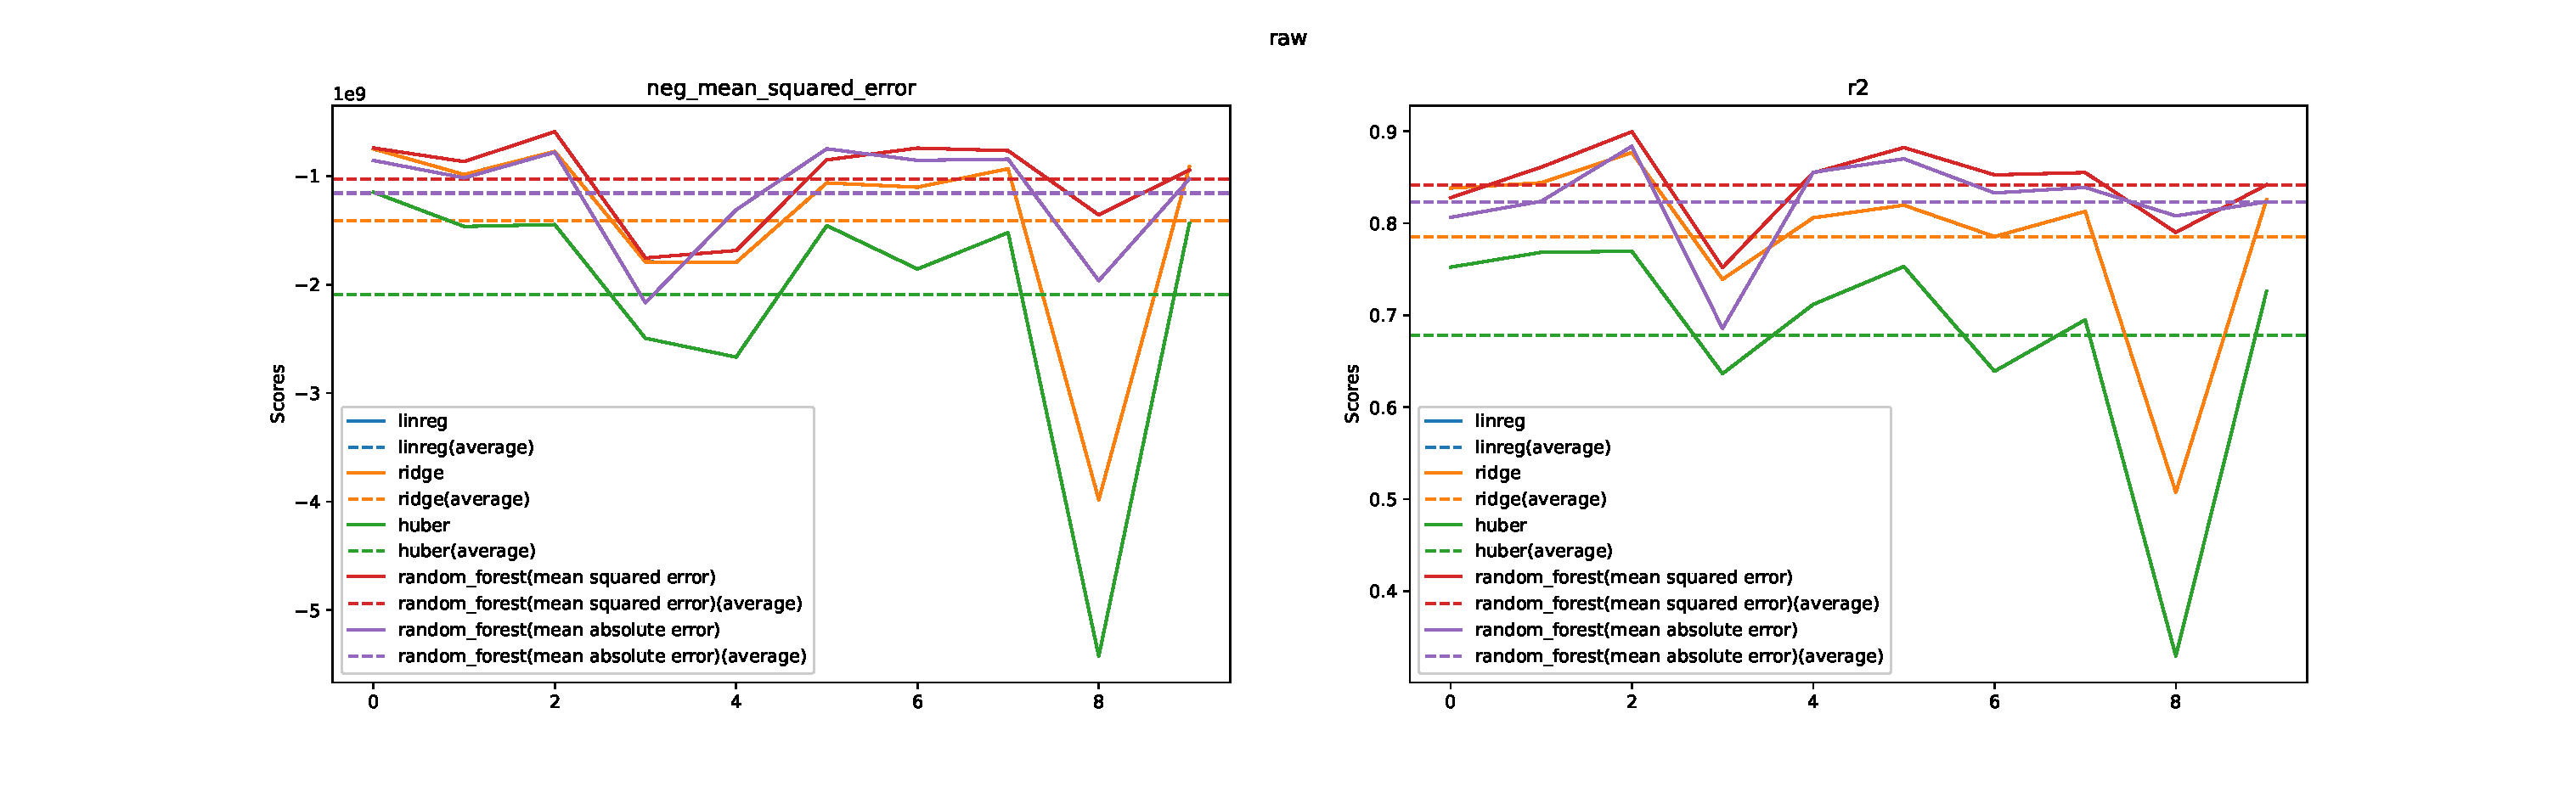
\includegraphics[width=0.9\textwidth]{plots/raw_model_scores}
\caption{Model scores without scaling}
\end{figure}

\begin{figure}[h]
\centering
\includegraphics[width=0.9\textwidth]{plots/randomized_42_model_scores}
\caption{Model scores with randomized data}
\end{figure}

\begin{figure}[h]
\centering
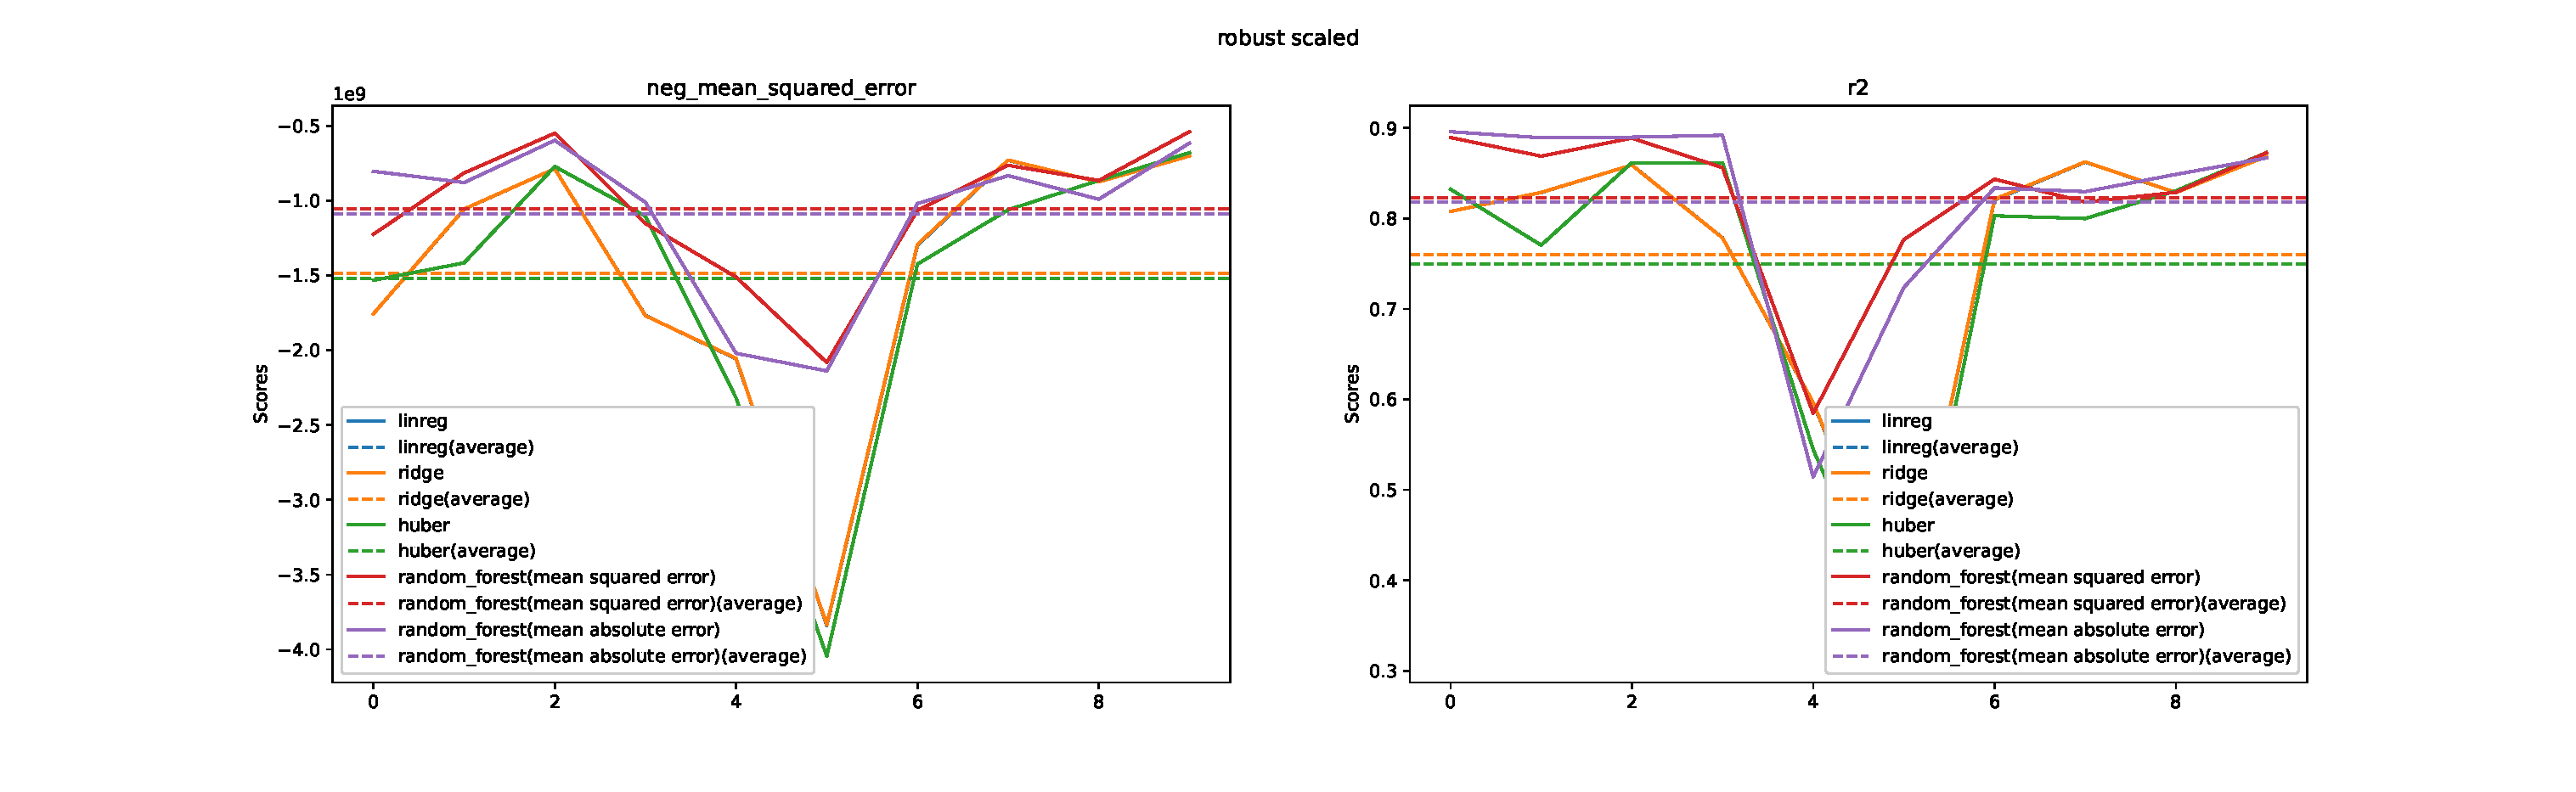
\includegraphics[width=0.9\textwidth]{plots/robust_scaled_model_scores}
\caption{Model scores with robust scaling}
\end{figure}

\begin{figure}[h]
\centering
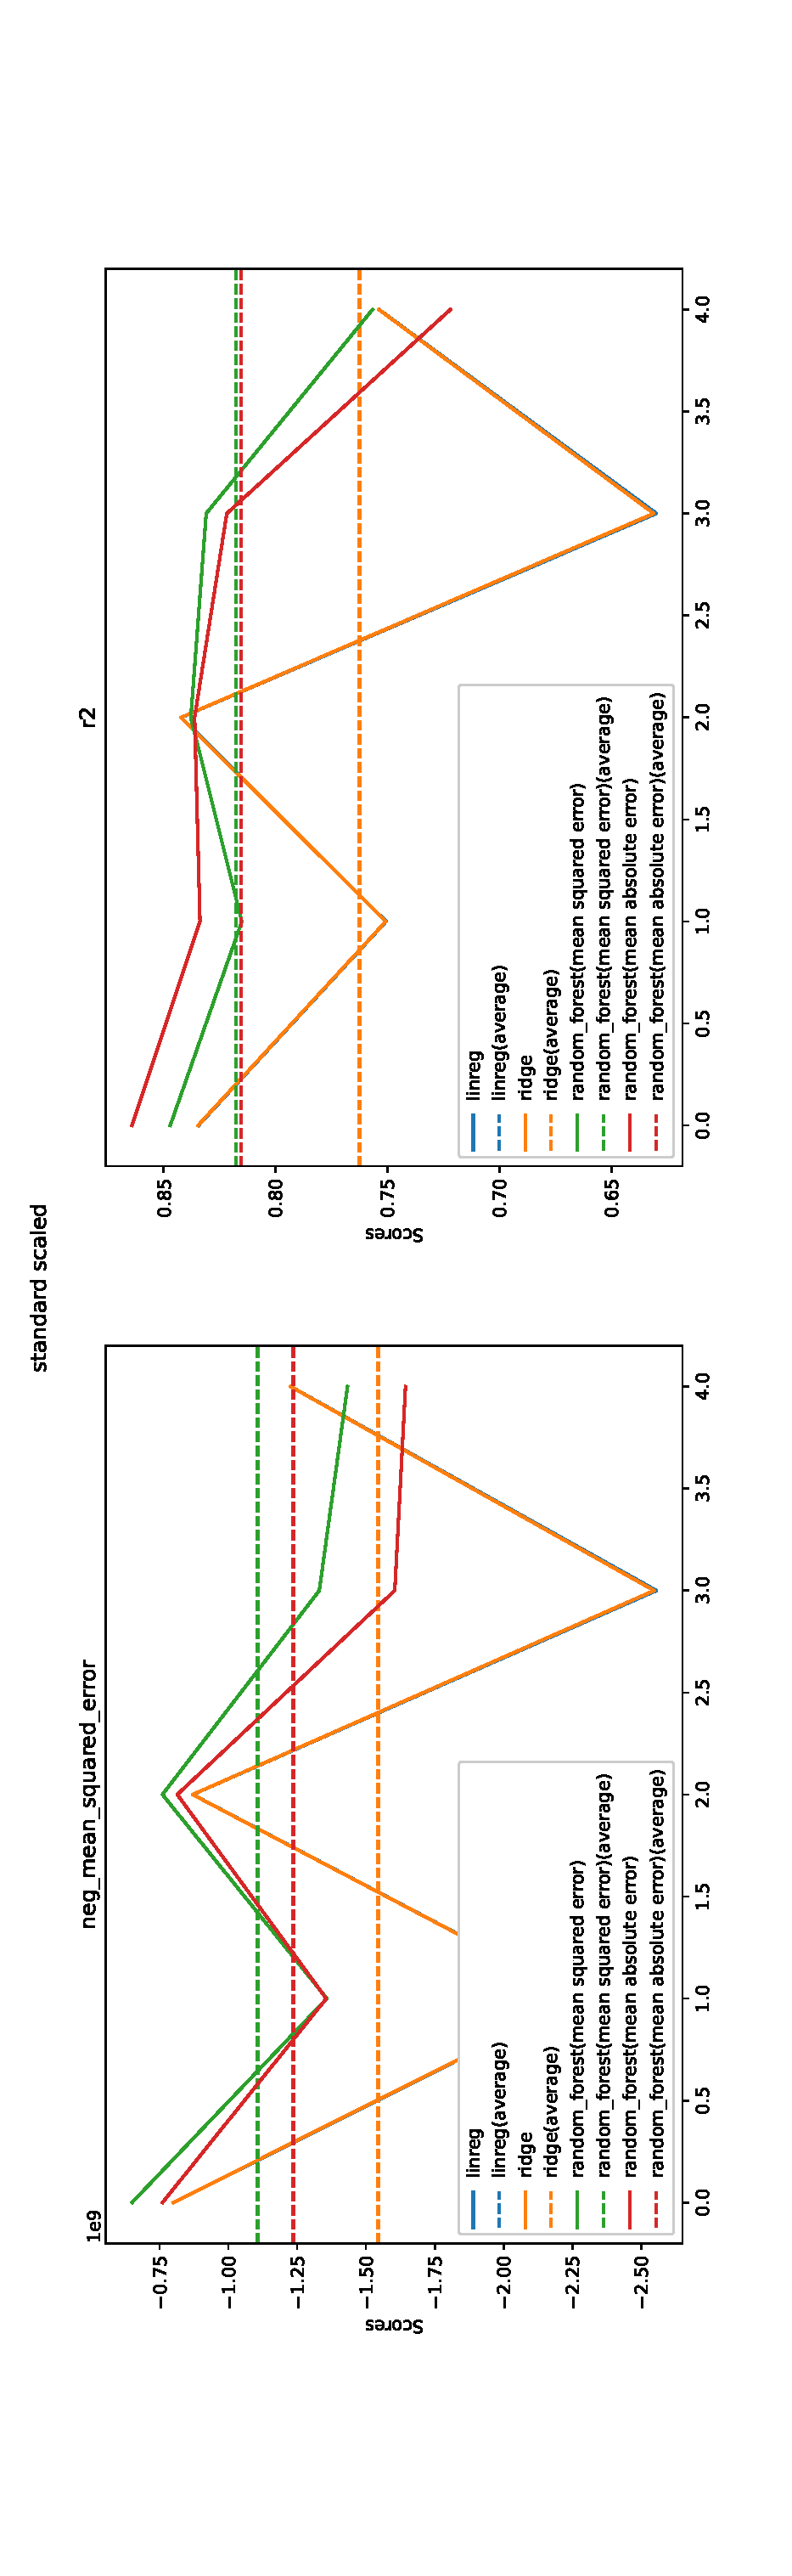
\includegraphics[width=0.9\textwidth]{plots/standard_scaled_model_scores}
\caption{Model scores with standard scaling}
\end{figure}

\begin{figure}[h]
\centering
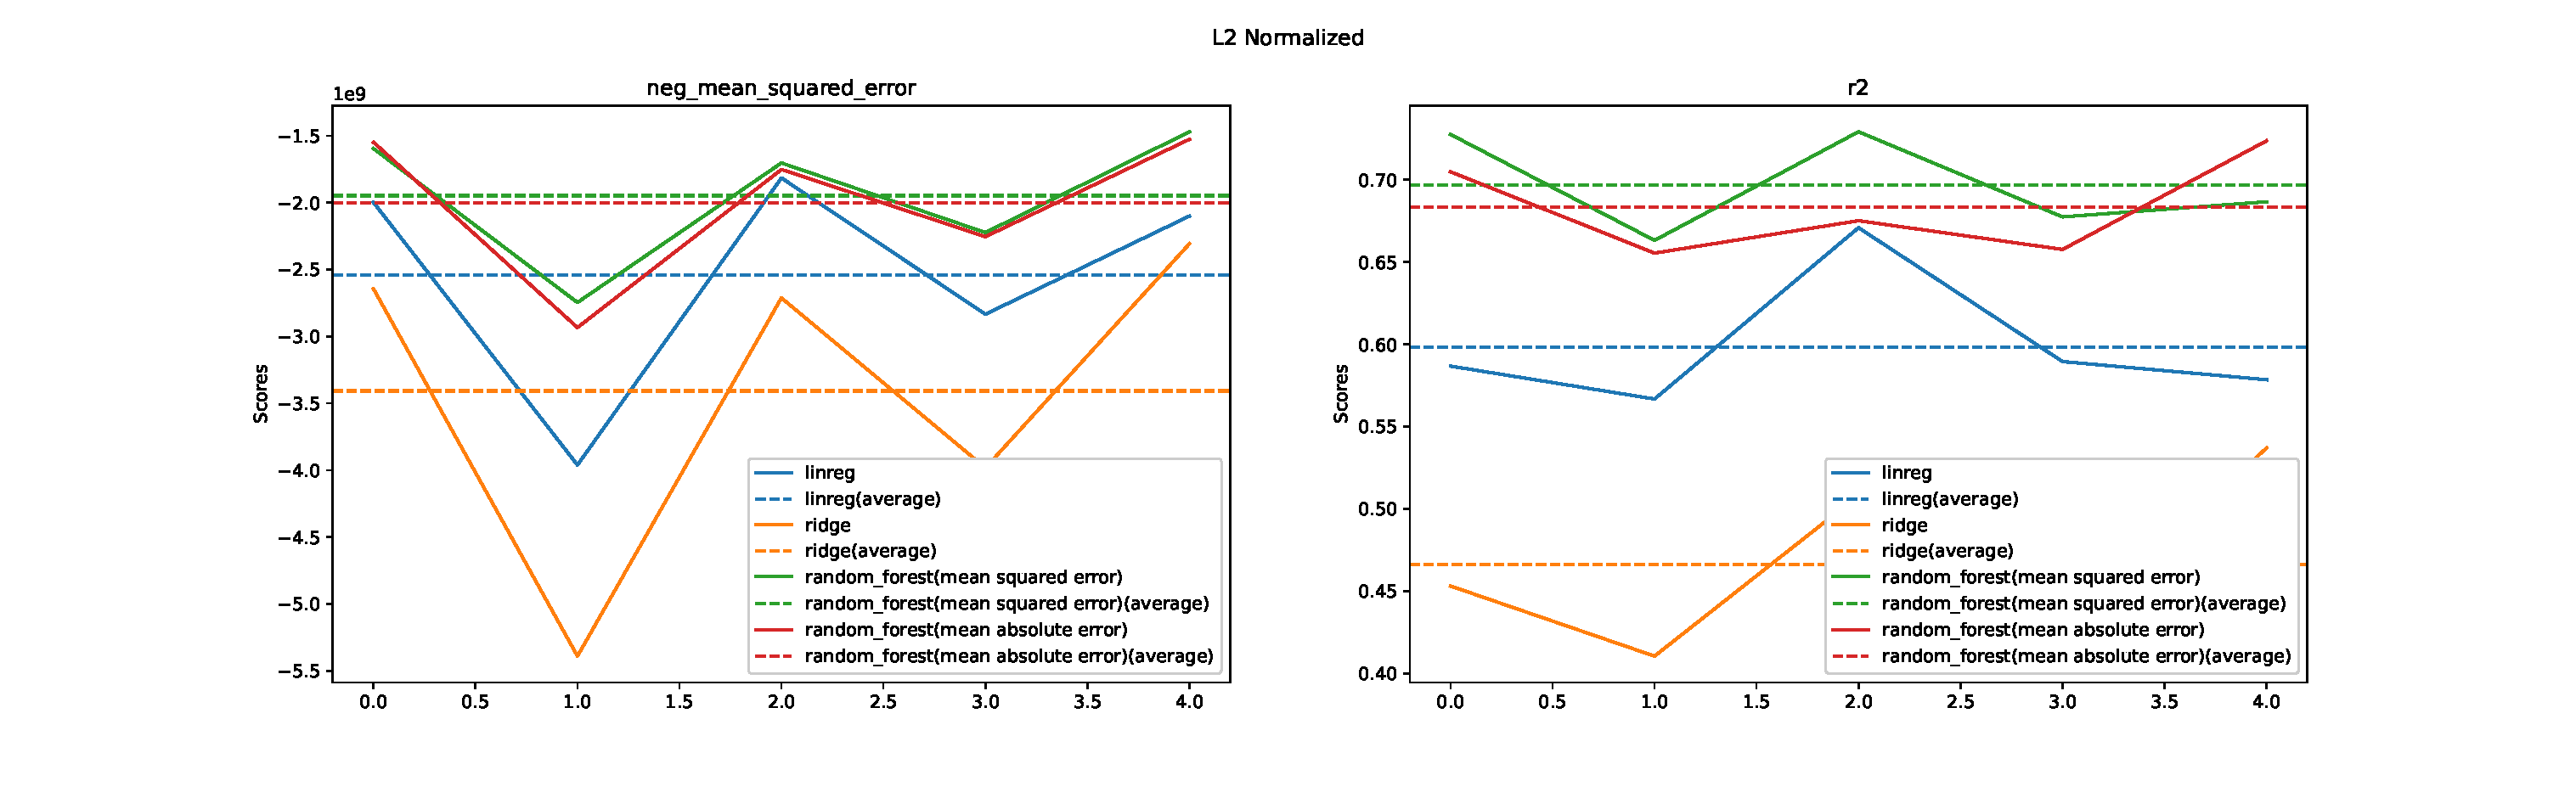
\includegraphics[width=0.9\textwidth]{plots/L2_Normalized_model_scores}
\caption{Model scores with L2 scaling}
\end{figure}

\begin{figure}[h]
\centering
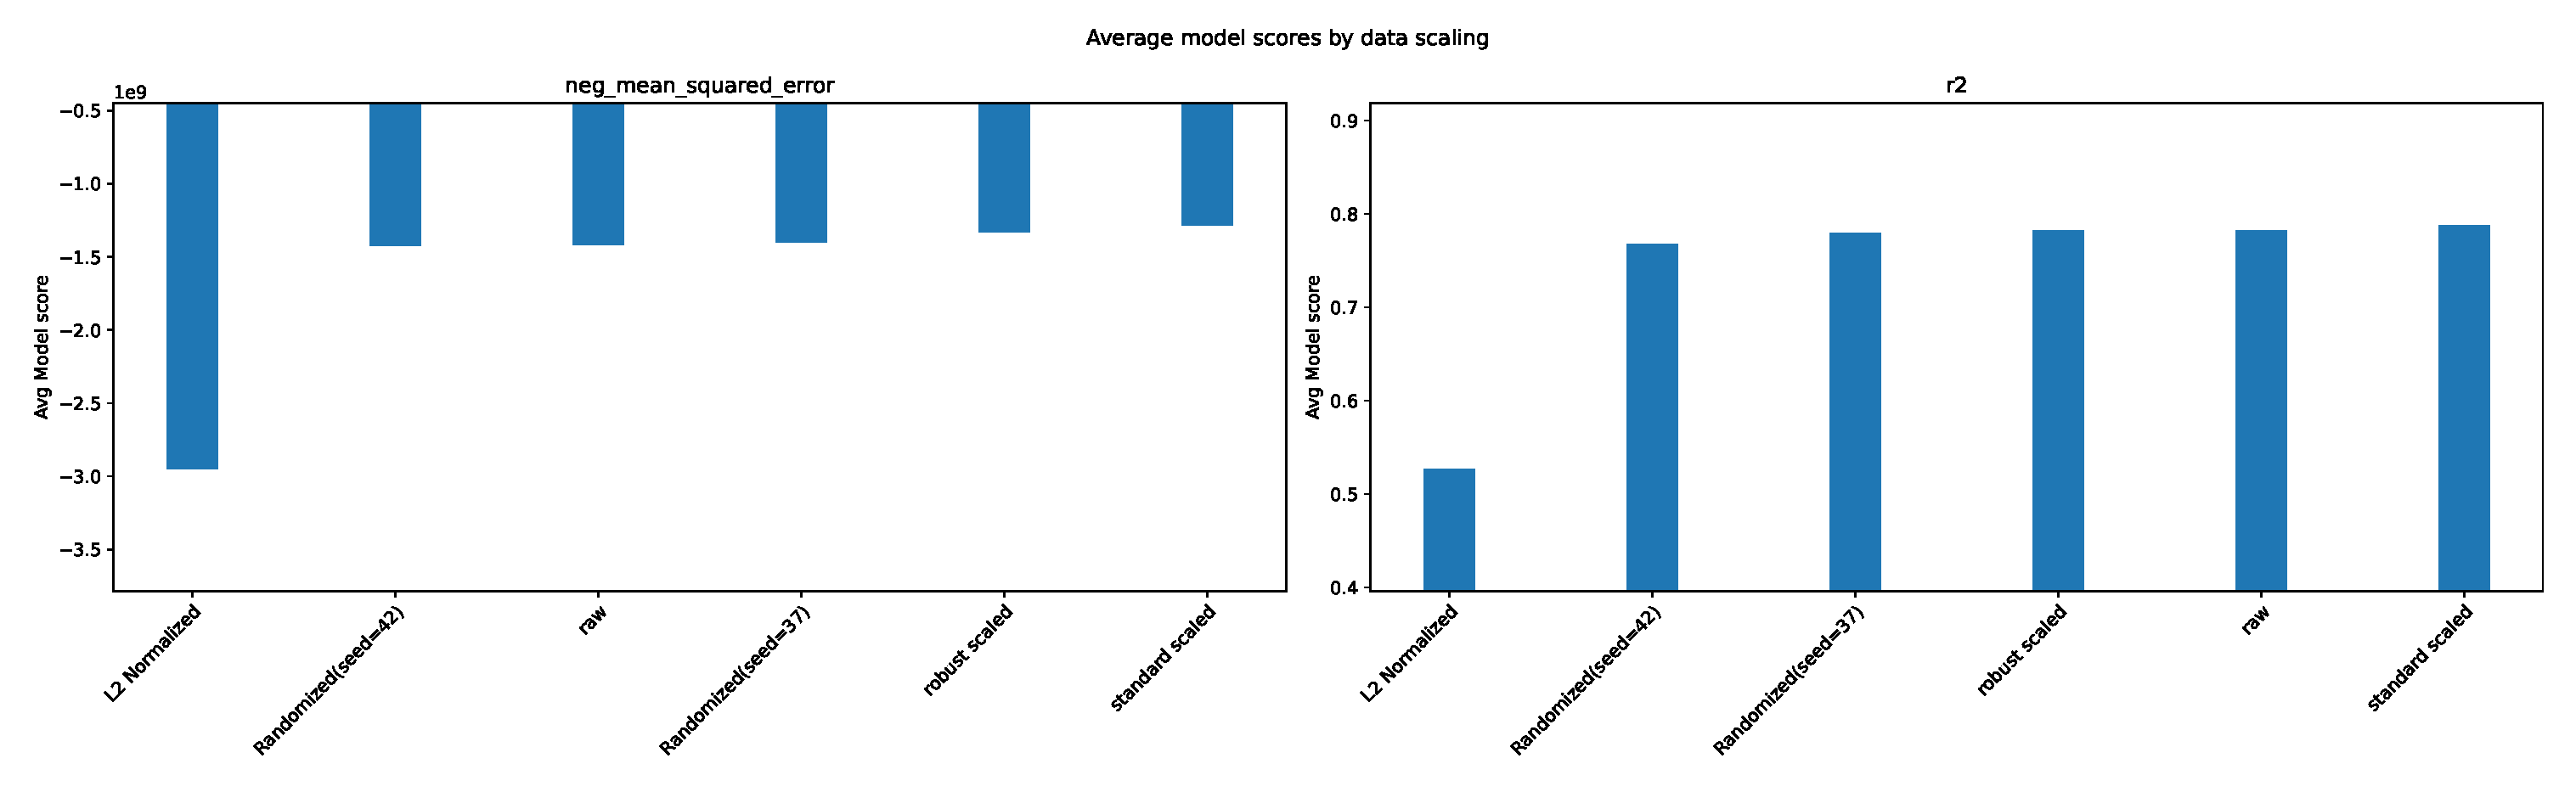
\includegraphics[width=0.9\textwidth]{plots/Average_model_scores_by_data_scaling_barcharts}
\caption{Average model scores by data scaling}
\end{figure}

\begin{figure}[h]
\centering
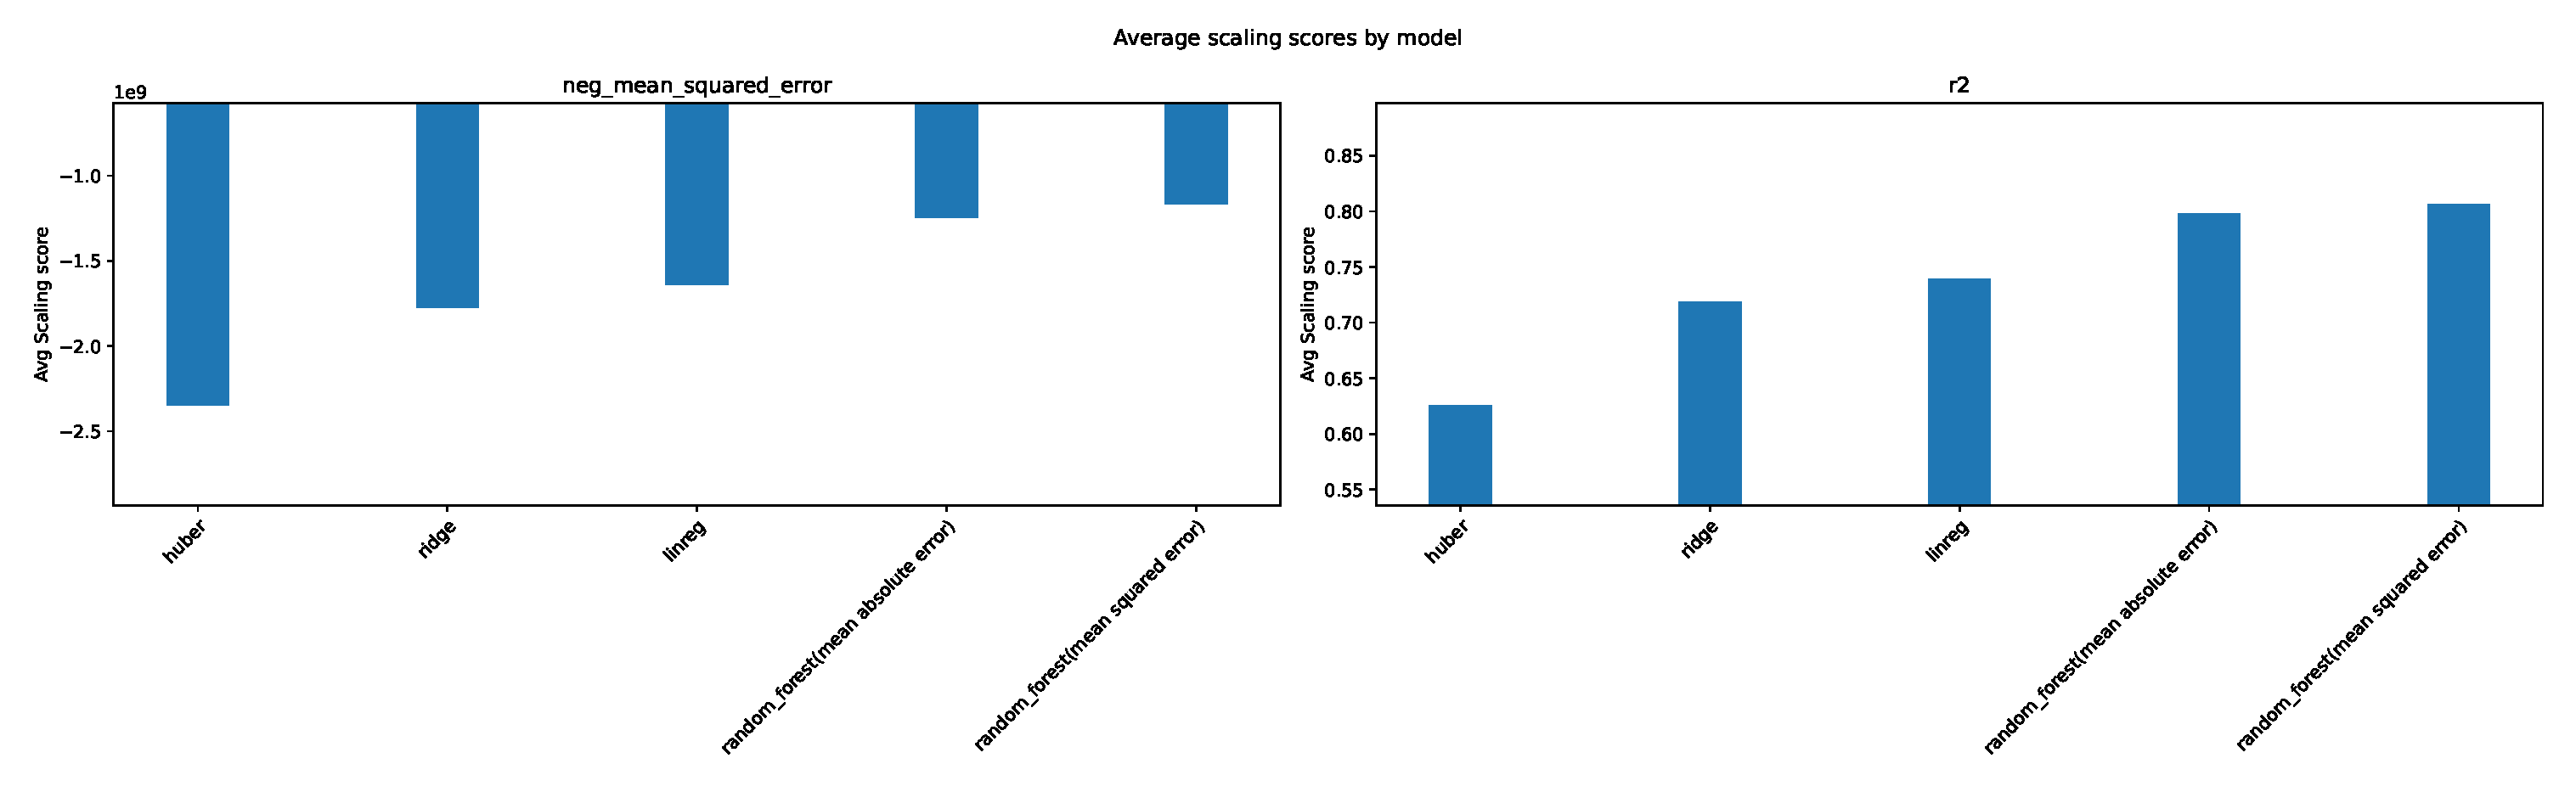
\includegraphics[width=0.9\textwidth]{plots/Average_scaling_scores_by_model_barcharts}
\caption{Average data scaling scores by model}
\end{figure}

\begin{figure}[h]
\centering
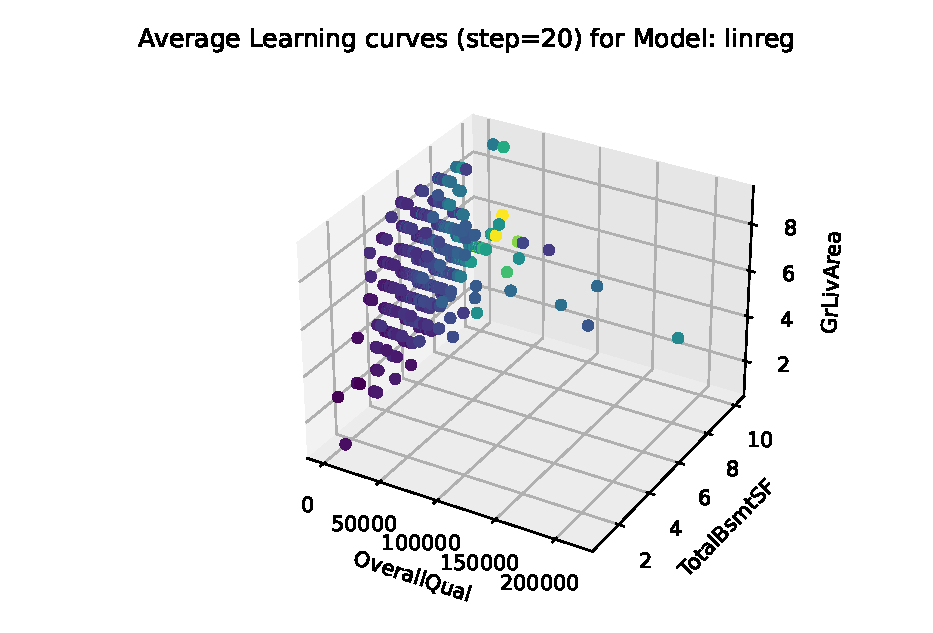
\includegraphics[width=0.8\textwidth]{plots/linreg_learning_curves}
\caption{Linear regression learning curve on standard scaled and variance filtered data}
\end{figure}

\begin{figure}[h]
\centering
\includegraphics[width=0.8\textwidth]{plots/random_forest_mse_learning_curves}
\caption{Random forest learning curve on standard scaled and variance filtered data}
\end{figure}

\begin{table}
\centering
\resizebox{.6\width}{!}{\begin{tabular}{lrrrr}
\toprule
{} &   Min &     Max &     Mean &     Std \\
\midrule
OverallQual &  1300 &  215245 &  10517.0 &  9978.0 \\
TotalBsmtSF &     1 &      10 &      6.0 &     1.0 \\
GrLivArea   &     1 &       9 &      6.0 &     1.0 \\
\bottomrule
\end{tabular}
}
\caption{Most important features (standard-scaled) as estimated by a random forest regressor using a mean squared error score.}
\end{table}

\end{document}